%
% unterteilung.tex
%
% (c) 2024 Prof Dr Andreas Müller
%
\begin{figure}
\centering
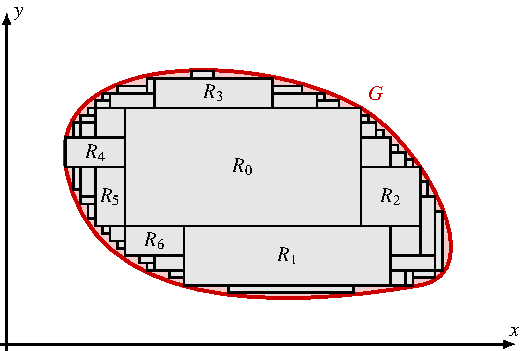
\includegraphics{chapters/040-felder/images/unterteilung.pdf}
\caption{Approximation eines Gebietes $G$ durch darin enthaltene Rechtecke
$R_0,R_1,\dots$.
Das Integral über das Gebebiet $G$ wird approximiert durch die Summe der
Integrale über die Rechtecke $R_k$.
\label{buch:felder:fig:unterteilung}}
\end{figure}
